Un ayuntamiento es responsable de mantener la siguiente red de carreteras. El número en cada arista es la longitud de la carretera en kilómetros.

\vspace{0.5cm} % Espacio vertical para separar el texto del gráfico

\begin{center}
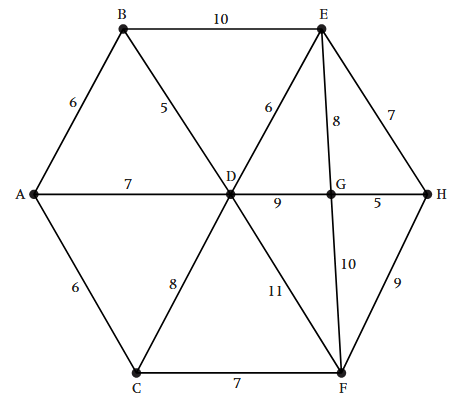
\includegraphics{ejercicios/carreteras_estado.png}

\end{center}

\vspace{0.5cm} % Espacio vertical

La oficina del ayuntamiento está ubicada en A.

\textbf{(a)} Un trabajador del ayuntamiento tiene que inspeccionar todas las carreteras, empezando y terminando en A. Encuentre la longitud de una ruta óptima.

\vspace{0.5cm} 

\textbf{(b)} Un supervisor, con base en A, también desea inspeccionar todas las carreteras. Sin embargo, el supervisor vive en H y desea comenzar su ruta en A y terminar en H. Encuentre la longitud de una ruta óptima para el supervisor.

